\scanpage{256}
diagramme de suites exactes
\diagram{\begin{tikzcd}[column sep=small,row sep=large]
(\uline{D}) & H^i(X_0,\mathbb Z)\arrow[r]\arrow[d,"u^i"] & R^if_*(\mathcal O_X)_y\arrow[r]\arrow[d,"v^i"] & R^if(\mathcal O_X^*)_y\arrow[r,dash,"\delta^i"]\arrow[d,"w^i"] & H^{i+1}(X_0,\mathbb Z)\arrow[r,"\alpha^{i+1}"]\arrow[d,"u^{i+1}"] & R^{i+1}f(\mathcal O_X)_y\arrow[d,"v^{i+1}"]\\
& H^i(X_0,\mathbb Z)\arrow[r,dash]\arrow[d] & {R^if(\mathcal O_X)_y}^{\wedge}\arrow[r,dash]\arrow[d] & \varprojlim H^i(X_n,\mathcal O_{X_n}^{\unsure{*|\wedge}})\arrow[r,dash,"\widehat\delta^i"]\arrow[d] & H^{i+1}(X_0,\mathbb Z)\arrow[r,"\widehat\alpha^{i+1}"]\arrow[d] & {R^{i+1}f(\mathcal O_X)_y}^{\wedge}\\
\deleted{0} & \deleted{H^i(X_0,\mathbb Z)}\arrow[r] & \deleted{H^i(X_0,\mathcal O_{\unsure{X_0}})_{\unsure{\mathrm{univ}|\mathrm{an}}}}\arrow[r] & \deleted{H^i(X_0,\mathcal O_{X_0}^*)_{\unsure{\mathrm{univ}|\mathrm{an}}}}\arrow[r] & \deleted{H^{i+1}(X_0,\mathbb Z)}\arrow[r] & \deleted{H^{i+1}(X_0,\mathcal O_{\unsure{X_0}})_{\unsure{\mathrm{univ}|\mathrm{an}}}}
\end{tikzcd}}
\figure{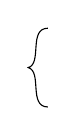
\begin{tikzpicture}[x=1cm,y=1cm]
\draw (0.25,1.1) .. controls (0,1.1) and (0.18,0.65) .. (0,0.6) .. controls (0.18,0.55) and (0,0.1) .. (0.25,0.1);
\end{tikzpicture}}

On en conclut, grâce au lemme des 5

a) $R^if_*(\mathcal O_X^*)_y\longrightarrow\varprojlim_n H^i(X_n,\mathcal O_{X_n}^{\unsure{\wedge|*}})$ est \uline{injectif}, et les \inserted{\unsure{deux mb ont $=$ images dans} $H^i(X_n,\mathcal O_{X_n}^*)$}

b) \unsure{Pour|Pourvu}

\uline{Corollaire} 1.6. \deleted{Supposons} que $R^if(\mathcal O_X)_y$ soit artinien, i.e. $y$ un pt isolé du supp $R^if(\mathcal O_X)$.
\deleted{Alors}\inserted{de sorte que}
\[
\inserted{\varinjlim_{U\ni y}H^i(f^{-1}(U),\mathcal O_U^*)=}
R^if_*(\mathcal O_X^*)\longrightarrow\varprojlim H^i(X_n,\mathcal O_{X_n}^{\unsure{\wedge|*}})
\]
soit un \uline{isomorphisme}.

\margin{\deleted{Comme le système projectif des}}
\margin{\unsure{Automatique} : pour $\unsure{n|i}$ grand \unsure{Niveau fini} $(X_0)$ est constant cad \unsure{inj} :
$\operatorname{Ker}(H^{i+1}(X_0,\mathbb Z)\longrightarrow R^{i+1}f_*(\mathcal O_X)_y)$}
\figure{\begin{tikzpicture}[x=1cm,y=1cm]
\draw (0,0) -- (0,2.5);
\draw[->] (-0.65,0.25) .. controls (-1.05,0.05) and (-0.8,-0.2) .. (-0.65,0.25);
\end{tikzpicture}}

c) \deleted{\unsure{Réciproquement}} Le lemme des 5 montre également que $R^if_*(\mathcal O_X^{\unsure{\wedge|*}})\longrightarrow\varprojlim H^i(X_n,\mathcal O_{X_n}^{\unsure{\wedge|*}})$ est toujours un \unsure{monomorphisme}.

\inserted{$\forall\xi\in\varprojlim H^i(X_n,\mathcal O_{X_n}^{\unsure{\wedge|*}})$, il existe un}
\deleted{des $(\unsure{H^i|R^i}(X_n,\mathcal O_{X_n}^*))_n$ \unsure{satisfont} M.L. (A.R.) \unsure{syst. proj.} \deleted{Comme les}}
\margin{Comme $v^{i+1}$ est injectif, $\operatorname{Ker}\alpha^{i+1}=\operatorname{Ker}\widehat\alpha^{i+1}$, \deleted{\unsure{pour}} donc $\operatorname{Im}\widehat\delta^i=\operatorname{Im}\delta^i$ donc pour}

\margin{\figure{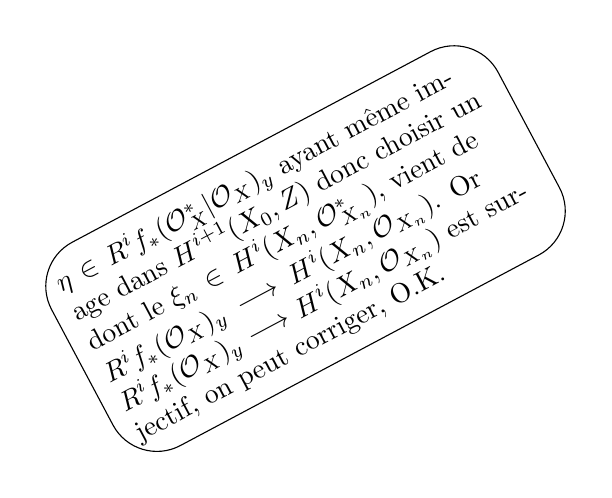
\begin{tikzpicture}
\node[draw,rounded corners=18pt,text width=6cm,align=left,rotate=28,inner sep=6pt] {
$\unsure{\eta}\in R^if_*(\unsure{\mathcal O_X^*|\mathcal O_X})_y$ ayant même image dans $H^{i+1}(X_0,\mathbb Z)$ \unsure{donc choisir un} \unsure{dont le} $\unsure{\xi_n}\in H^i(X_n,\mathcal O_{X_n}^*)$, \unsure{vient de}
\(R^if_*(\mathcal O_X)_y\longrightarrow H^i(X_n,\mathcal O_{X_n})\).
\uuline{Or} $R^if_*(\mathcal O_X)_y\longrightarrow H^i(X_n,\mathcal O_{X_n})$ est surjectif, on peut corriger, O.K.
};
\end{tikzpicture}}}

Le cas le plus important pour nous est celui où $i=1$, qui donne le

\figure{\begin{tikzpicture}\draw (0,0) -- (0,4.4);\end{tikzpicture}}

\uline{Th.} 1.\deleted{\unsure{8}}\inserted{7}. Soit $f:X\longrightarrow Y$ une application propre d'espaces analytiques \uline{sur} $\mathbb C$, $y\in Y$, \inserted{$Y_n=\operatorname{Specan}\mathcal O_y/\mathfrak m_y^{n+1}$,} $X_n=X\times_Y Y_n$, \deleted{Alors} posons
\[
\operatorname{Pic}(X_y)=\varinjlim_{U\ni y}\operatorname{Pic}(f^{-1}(U))
=R^1f(\mathcal O_X^{\unsure{\wedge|*}})_y,
\]
\deleted{Alors considérons l'hom}
\[
\operatorname{Pic}(\widehat X_y)=\varprojlim_n\operatorname{Pic}(X_n).
\]
\mspage{255}
